\documentclass[11pt]{article}
\usepackage[T1]{fontenc}
\usepackage[margin=25mm]{geometry}
\usepackage{amsmath,amssymb,graphicx,booktabs,longtable,array,microtype}
\usepackage[font=small]{caption}
\usepackage[section]{placeins}
\usepackage[backend=biber,style=numeric-comp,sorting=none,maxbibnames=12]{biblatex}
\usepackage{authblk}
\addbibresource{references.bib}
\usepackage{xurl}
\usepackage[hidelinks]{hyperref}
\graphicspath{{figures/}}
\renewcommand{\thesection}{S\arabic{section}}
\renewcommand{\thefigure}{S\arabic{figure}}
\renewcommand{\thetable}{S\arabic{table}}
\renewcommand{\theequation}{S\arabic{equation}}
\setlength{\parskip}{4pt}
\setlength{\parindent}{0pt}
% Authors and affiliations (confirm with all authors before submission).
\title{When Scientific Measurements Mislead Language Models:\\
Definition-Aware Verification of Atomistic Evidence\\[0.45em]\large Supplementary Information}
\author[1]{Obed Issakah}
\author[2]{Md Khirul Alam Titu}
\author[2]{Srivathsan Badrinarayanan}
\author[1]{Ravi F. Saraf}
\author[1]{Janghoon Ock\thanks{Corresponding author: \texttt{jock2@unl.edu}}}
\affil[1]{Department of Chemical and Biomolecular Engineering, University of Nebraska--Lincoln, Lincoln, NE 68588, USA}
\affil[2]{Department of Chemical Engineering, Carnegie Mellon University, 5000 Forbes Avenue, Pittsburgh, PA 15213, USA}
\renewcommand\Authfont{\small}
\renewcommand\Affilfont{\small}
\setlength{\affilsep}{0.5em}
\date{}

\begin{document}
\maketitle
\noindent\textbf{Scope.} This document supports the unified GeoScope evidence-verification study. It documents the 55-system UMA-relaxed and 48-system OC20 trajectory source collections, their shared proof definitions, and source-specific verification and confidence analyses. The separately archived per-figure data and scripts are distributed as \texttt{publication\_figures.zip} (not included in this manuscript-source package). Frozen model results were not changed. The original 55-system coordinate table was unavailable for rebuilding the earlier scatterplot, so Fig.~S1 shows only its reported summary values. Independent chemical review is still pending.

\section{Supplementary Methods}
\subsection{Measurement definitions and physical admissibility}
A distance has scientific meaning only when we know which atoms and structures it describes. Let $\mathbf r_i^{(0)}$ and $\mathbf r_i^{(1)}$ be the positions of atom $i$ in the first and second stored structures. Let $S$ be a chosen set of atoms and $n_S$ its number of atoms. The stored-frame root-mean-square deviation (RMSD) is
\begin{equation}
 R_S=\left[\frac{1}{n_S}\sum_{i\in S}\left\|\operatorname{MIC}(\mathbf r_i^{(1)}-\mathbf r_i^{(0)})\right\|^2\right]^{1/2}.
 \label{eq:si_frame}
\end{equation}
Here $R_S$ is the RMSD for set $S$. The symbol $\sum$ means add over the atoms in $S$, and $\|\cdot\|$ is vector length. The function $\operatorname{MIC}$ chooses the shortest equivalent displacement through the periodic simulation cell. We use matching atom identities at both endpoints.

For the adsorbate set $S_A$, the stored-frame RMSD is $A=R_{S_A}$. For the mobile-atom set $S_M$, it is $M=R_{S_M}$. Fixed atoms are checked separately. These quantities keep motion relative to the stored surface coordinates. In contrast, internal adsorbate RMSD $I$ measures change of shape after periodic unwrapping and fitting one structure to the other by rotation and translation. The fit uses a proper Kabsch rotation and does not reflect the molecule.\cite{kabsch1978discussion} Thus a molecule can move across a surface with a large $A$ but small $I$. The procedure uses a geometric rule to guess bonds; that rule has not been checked for every system by an independent chemist.

When the adsorbate atoms are part of the mobile set ($S_A\subset S_M$), both RMSDs use the same structure pair, periodic handling, and equal atom weights. We can then write
\begin{equation}
 M^2=\frac{n_A A^2+\sum_{i\in S_M\setminus S_A}\|\mathbf d_i\|^2}{n_M},
 \qquad
 M\geq\sqrt{\frac{n_A}{n_M}}\,A,
 \qquad
 A\leq\sqrt{\frac{n_M}{n_A}}\,M.
 \label{eq:si_bounds}
\end{equation}
Here $n_A$ is the number of adsorbate atoms, $n_M$ is the number of mobile atoms, and $\mathbf d_i=\operatorname{MIC}(\mathbf r_i^{(1)}-\mathbf r_i^{(0)})$ is the displacement of atom $i$. The set $S_M\setminus S_A$ contains mobile atoms that are not part of the adsorbate. All squared distances are nonnegative, so the remaining mobile atoms cannot lower the sum below the adsorbate contribution. These bounds do not apply to $I$, to a different structure pair, or to different measurement rules.

A licensed proof uses a measurement and mathematical operation that match the claim's atom set, structure pair, frame, alignment, periodic treatment, weights, and units. A lucky correct verdict with mismatched evidence is still an invalid proof.

\subsection{UMA-relaxed source collection: design and frozen sample}
The original study used OC20-Dense starting geometries with UMA \texttt{uma-s-1p2p1} and ASE FIRE relaxation. Initial and final positions of 55 qualifying source groups were retained after convergence and geometric checks (from 60 attempted groups). Twenty development groups had been excluded before final selection, and source selection was fixed using seed 20261021. The source qualification checked atom identity, constraints, cell, periodic flags, force convergence, fixed atoms, and stability of a heuristic adsorbate graph. Each accepted geometry also supplied a synthetic adsorbate translation control, explicitly distinguished from a physical relaxation.\cite{chanussot2021open,wood2025uma,larsen2017atomic}

The benchmark comprised 1,760 claim variants: 550 supported, 550 contradicted, and 660 insufficient-evidence. Thus 1,100 cases were answerable. Original three-model inference used one response for each direct-answer and evidence-selection prompt per variant. The deterministic arithmetic-only, comparison-ID and full-definition checkers were applied to the \emph{same} evidence selections; no check retrieved replacement evidence. The exhaustive enumerator reproduced all labels by construction when every public record and rule was supplied.

\begin{table}[htbp]\centering\small
\caption{Original-study sample and Qwen proof-checking results.}
\begin{tabular}{lr}\toprule Quantity&Count\\\midrule
Qualified UMA-relaxed source groups&55\\
All benchmark cases&1760\\
Answerable cases&1100\\
Insufficient-evidence cases&660\\
Qwen full-definition licensed numerical answers&312\\
Qwen additional comparison-ID acceptances rejected&81\\
Of those, wrong verdict / correct verdict but invalid proof&42 / 39\\
\bottomrule\end{tabular}
\end{table}

Original-study counts come from the frozen Phase 3 report. The complete original 10,560 responses were not rescored in the Phase 4 audit.

\subsection{OC20 trajectory source collection: validation gate}
The external study instead used the OC20 IS2RE/IS2RS \texttt{val\_ood\_both} per-system relaxation trajectories, not interleaved S2EF snapshot batches.\cite{chanussot2021open} The official archive download was checked against published MD5 \texttt{bc74b6474a13542cc56eaa97bd51adfc}. Its selected file hashes and selection order are preserved in the source gate. A SHA-based fixed order admitted 48 unique systems among the first 49 examined; this does not estimate the whole-dataset acceptance rate. One candidate was rejected for synthetic-control graph inconsistency. Each qualified pair uses the first and last \emph{stored} trajectory frame, not necessarily a fully relaxed minimum; the control is a synthetic comparison, not a second DFT trajectory. There are 16 base claims per physical source group and two evidence presentations per claim. Thus the external benchmark contains $48\times16\times2=1536$ questions with 480 supported, 480 contradicted, and 576 insufficient-evidence outcomes. Paired presentations were kept together when sharding the workload.

Independent recomputation checked 144 shared-frame RMSD values (mobile, adsorbate and fixed, three per system), and separately recalculated all 48 aligned internal adsorbate RMSDs; agreement was within numerical precision. A separately implemented proof checker reproduced all 768 structured reference proof lists. The paired 768 written-rendering cases had matching verdicts and allowed operation classes; alias IDs differ by presentation. These reproducibility checks do \emph{not} independently validate the bond heuristic, the scientific adequacy of every proof axiom, or model-pretraining exclusion.

\begin{table}[htbp]\centering\small
\caption{External OC20 source gate and benchmark sizes.}
\begin{tabular}{lr}\toprule Quantity&Count\\\midrule
Selected physical source systems&48\\
Candidates screened before target reached&49\\
Structures with independently reproduced internal RMSD&48\\
Paired scientific base cases&768\\
Structured questions / written reports&768 / 768\\
Supported / contradicted / insufficient cases&480 / 480 / 576\\
Questions per model / total four-model predictions&1536 / 6144\\
\bottomrule\end{tabular}
\end{table}

\subsection{Model output parsing and proof evaluation}
Four frozen open-weight checkpoints were evaluated: Qwen3-4B-Instruct-2507, Phi-4-mini-instruct, SmolLM3-3B, and Qwen3-32B-AWQ. The 32B model uses four-bit quantized weights and a separate inference backend; cross-model differences are not a controlled model-size intervention. Strict parsing required the declared single-evidence JSON form with no enclosing code fence. Fence-normalized parsing removes only an outer Markdown code block; it does not change the model's evidence ID, operation or verdict. The frozen operation-only repair enumerates alternative licensed operations \emph{for the model-selected evidence ID}; it is an oracle-assisted diagnostic, not proof of a deployable tool or of improved intrinsic model reasoning. Neither a malformed selection nor a verifier rejection counts as a correct scientific abstention.

\subsection{Confidence replay and statistical interpretation}
All 6,144 external questions were replayed with per-token probability extraction. Every replay matched its original output exactly. For each answer, we locate the generated tokens for its selected evidence ID and operation. The decision-token score is their geometric mean:
\begin{equation}
 G=\exp\!\left(\frac{1}{|T|}\sum_{t\in T}\log p_t\right),
\end{equation}
Here $G$ is the score, $T$ is the set of chosen decision tokens, $t$ labels one token, $|T|$ counts those tokens, and $p_t$ is the probability assigned by the model to token $t$. The function $\log$ is the natural logarithm, and $\exp$ reverses that logarithm. $G$ measures likelihood of generated text, not the probability that the scientific proof is correct. AUROC measures how well $G$ orders correct versus incorrect proof selections among answerable cases. Top-decile performance retains the highest-confidence 10\% of eligible answers per model. Availability was 960/960, 918/960, 735/960 and 960/960 for Qwen3-4B, Phi, SmolLM and Qwen3-32B, respectively. Missing decision spans are excluded transparently, not imputed. These retrospective analyses are \emph{not} independent deployment-threshold calibration. Raw per-token log-probability vectors were not archived; the frozen span summaries and extraction code were retained.

\subsection{Uncertainty and dependency between cases}
Original-study intervals used 1,000 bootstrap resamples of the 55 complete source groups (seed 20261021), with all prompts and paired cases from a group kept together. Phase 4 external and confidence intervals resampled the 48 complete external source groups; the confidence package used 1,200 source-group bootstrap replicates. Percentile 95\% intervals are descriptive. They do not account for unknown model pretraining overlap or broader benchmark selection bias. Unadjusted multiple exploratory comparisons should not be presented as independent confirmatory effects.

\section{Supplementary Figures: UMA-relaxed Source Collection}
\begin{figure}[htbp]\centering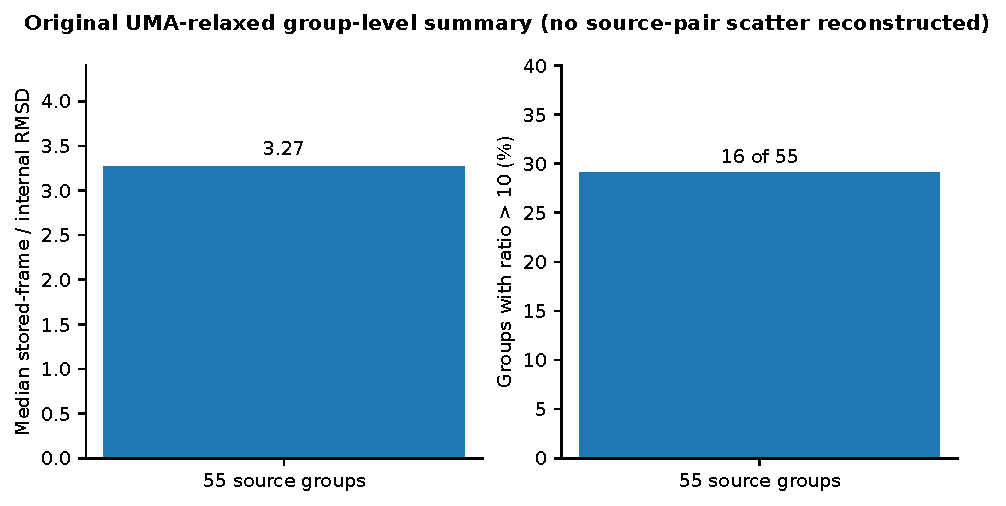
\includegraphics[width=.85\linewidth]{figure_S01.pdf}\caption{Stored-frame adsorbate and rigid-aligned internal RMSD for all 55 qualified UMA-relaxed systems. Each point is an original archived measurement; the dashed equality line is descriptive, not a licensed scientific bound.}\label{fig:si_physical}\end{figure}
\begin{figure}[htbp]\centering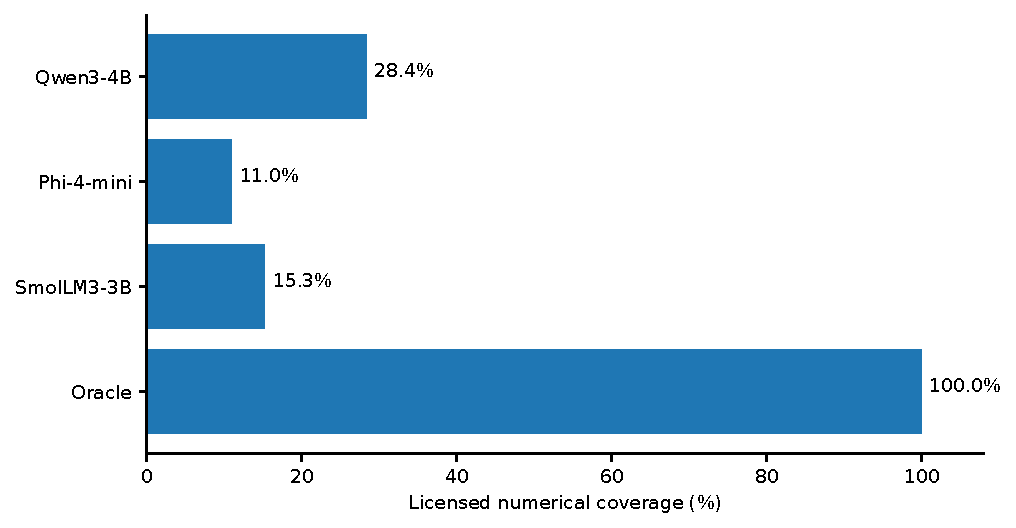
\includegraphics[width=.89\linewidth]{figure_S02.pdf}\caption{Licensed numerical-answer coverage in the original study.}\label{fig:si_coverage}\end{figure}
\begin{figure}[htbp]\centering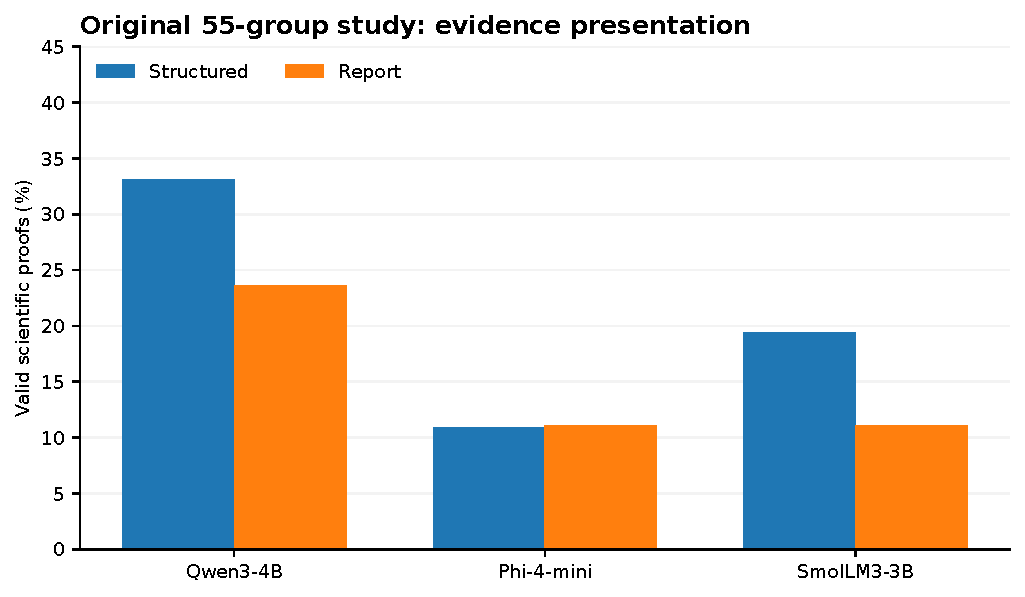
\includegraphics[width=.90\linewidth]{figure_S03.pdf}\caption{Licensed-answer coverage by evidence presentation in the original study.}\label{fig:si_presentation}\end{figure}
\begin{figure}[htbp]\centering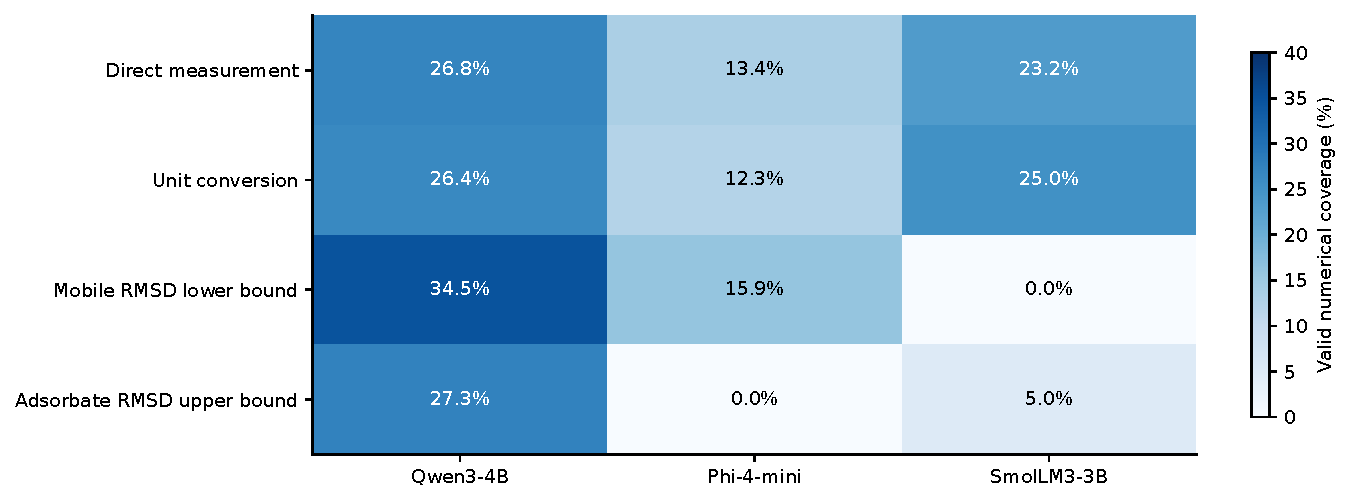
\includegraphics[width=\linewidth]{figure_S04.pdf}\caption{Licensed-answer coverage by claim family in the original study.}\label{fig:si_families}\end{figure}

\section{Supplementary Figures: OC20 Trajectory Source Collection}
\begin{figure}[htbp]\centering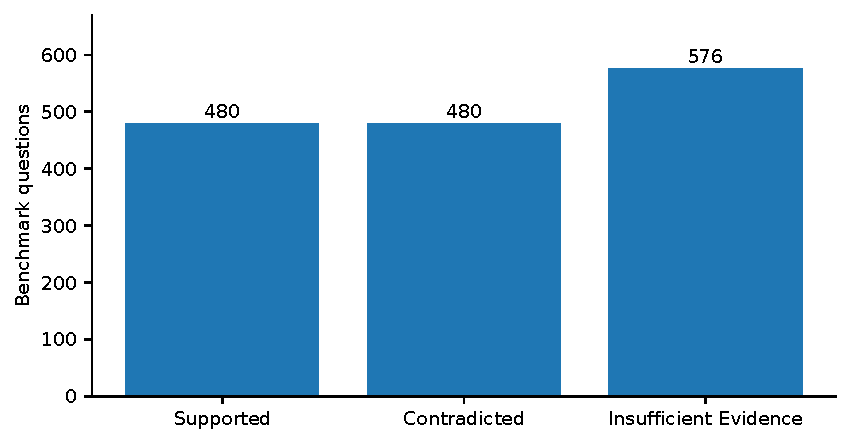
\includegraphics[width=.84\linewidth]{figure_S05.pdf}\caption{Reference verdict counts for the external OC20 benchmark.}\label{fig:si_balance}\end{figure}
\begin{figure}[htbp]\centering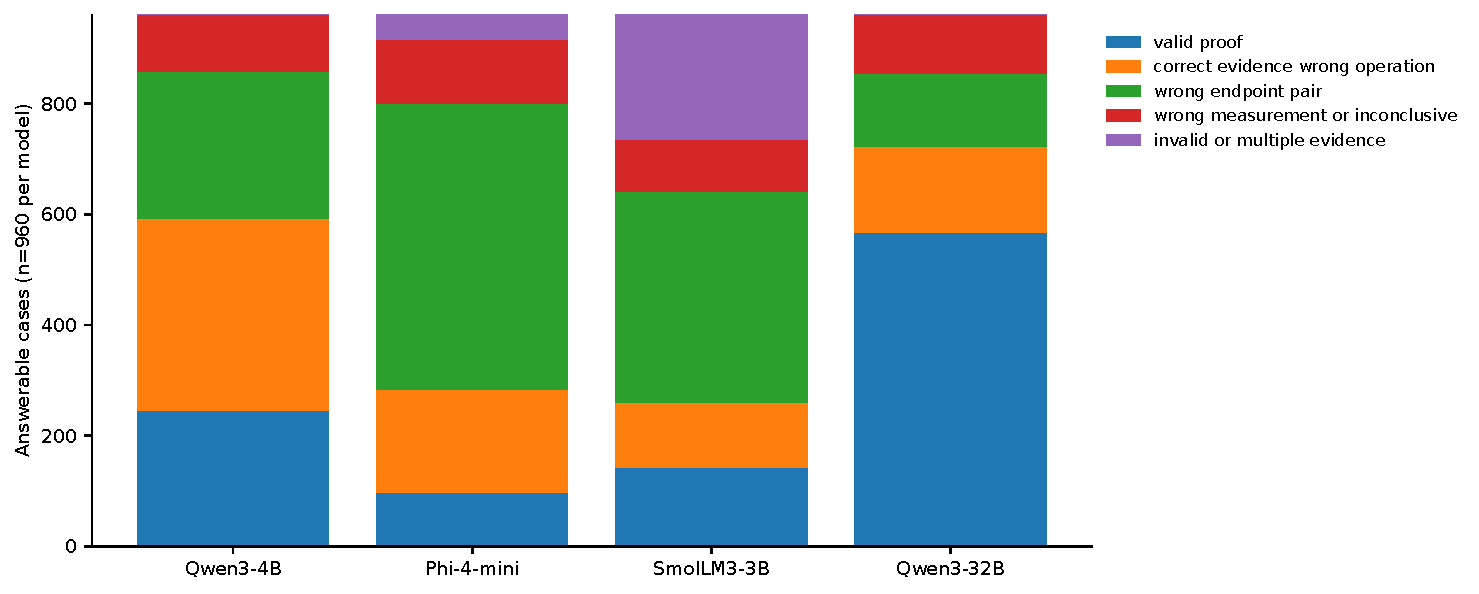
\includegraphics[width=\linewidth]{figure_S06.pdf}\caption{Valid proofs and error types for four models on external OC20 questions.}\label{fig:si_errors}\end{figure}
\begin{figure}[htbp]\centering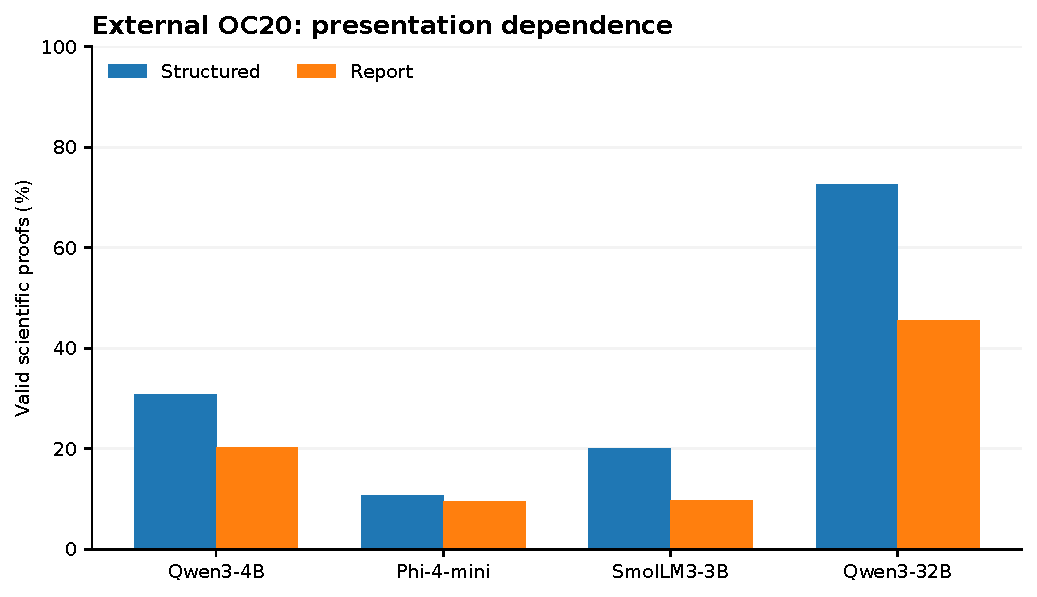
\includegraphics[width=\linewidth]{figure_S07.pdf}\caption{External OC20 proof validity by evidence presentation.}\label{fig:si_external_presentation}\end{figure}

\section{Supplementary Figures: Confidence and Cross-Collection Comparison}
\begin{figure}[htbp]\centering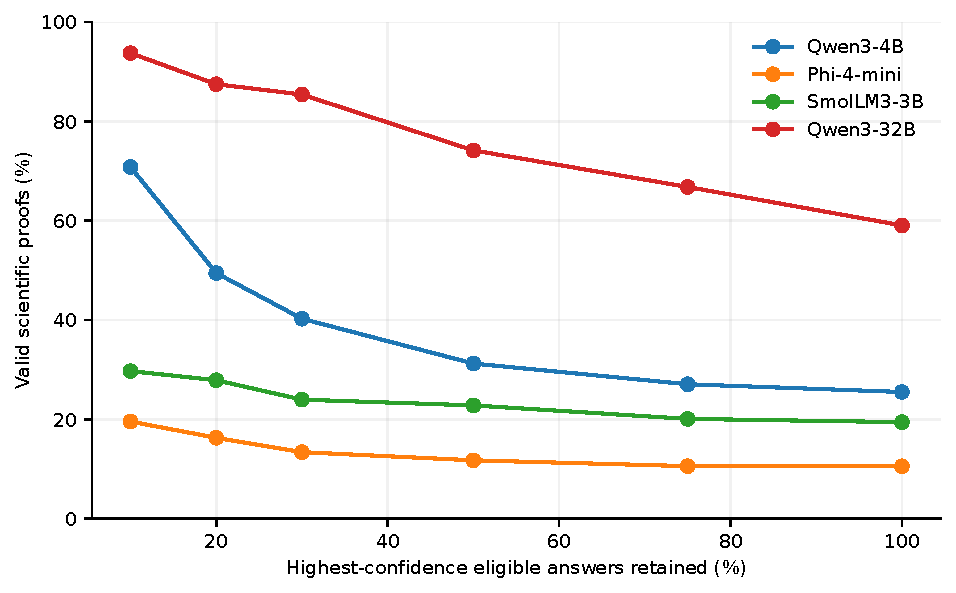
\includegraphics[width=.93\linewidth]{figure_S08.pdf}\caption{Proof accuracy as lower-confidence answers are excluded.}\label{fig:si_selective}\end{figure}
\begin{figure}[htbp]\centering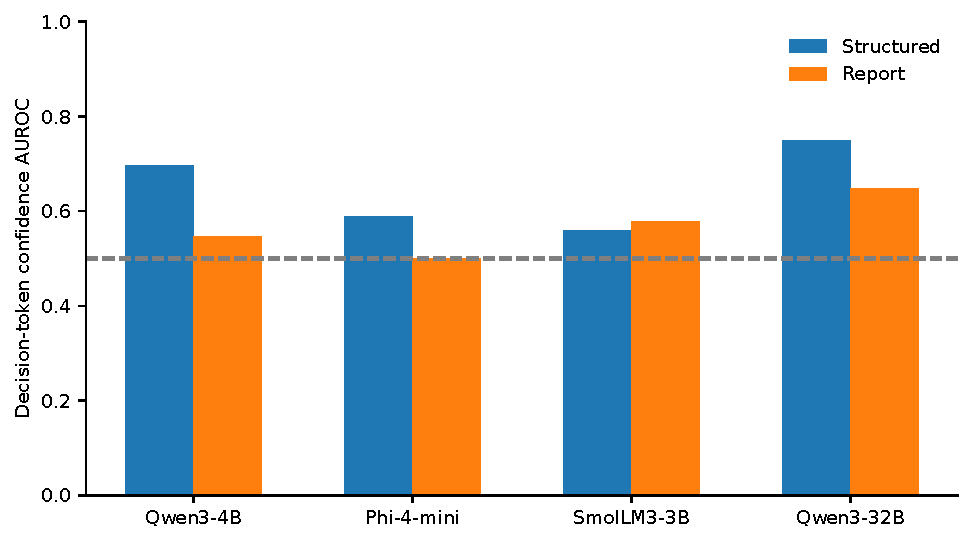
\includegraphics[width=.90\linewidth]{figure_S09.pdf}\caption{Decision-token confidence AUROC by evidence presentation.}\label{fig:si_conf_presentation}\end{figure}
\begin{figure}[htbp]\centering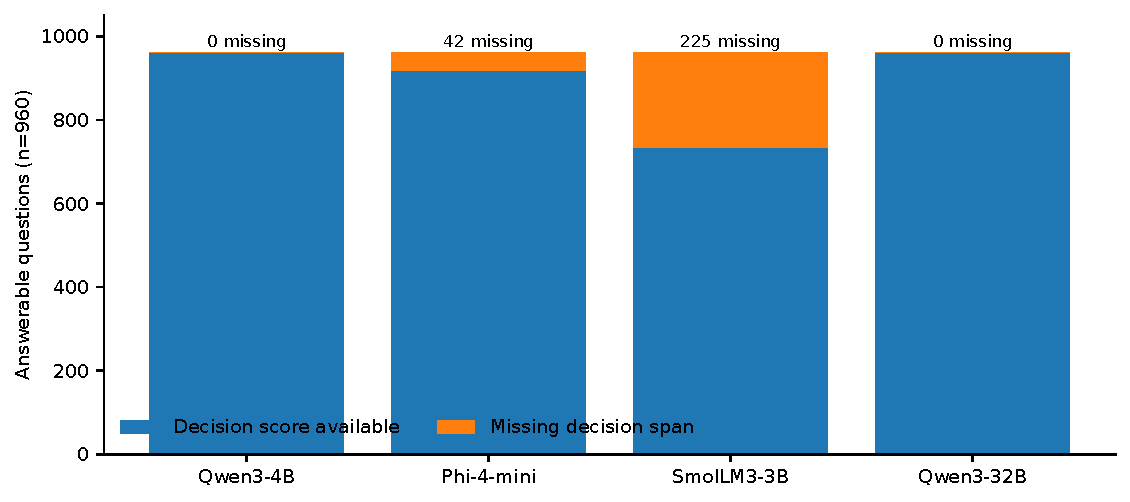
\includegraphics[width=.90\linewidth]{figure_S10.pdf}\caption{Decision-token score availability on the 960 answerable external questions per model; insufficiency recognition is evaluated separately.}\label{fig:si_missing}\end{figure}
\begin{figure}[htbp]\centering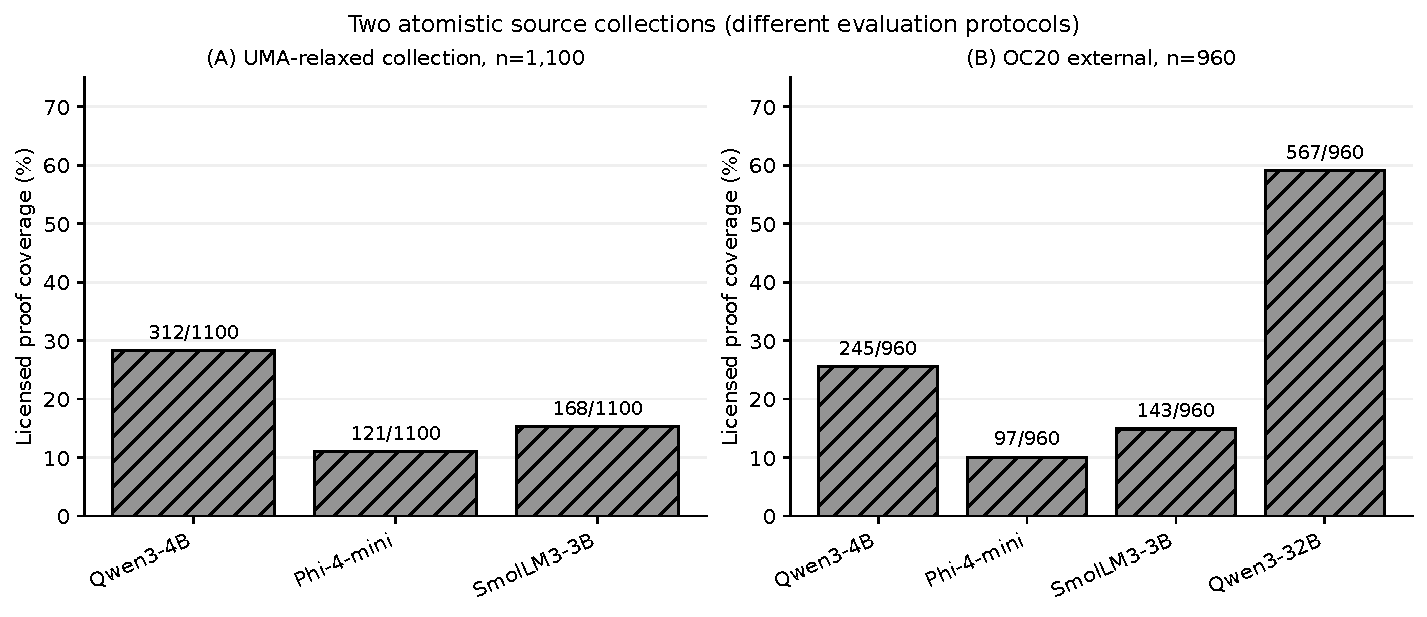
\includegraphics[width=\linewidth]{figure_S11.pdf}\caption{Full-definition licensed proof coverage on the 55-system UMA collection (three evaluated models) and fence-normalized coverage on the 48-system OC20 collection (four models). Their different source populations and scoring conventions prevent a controlled performance comparison.}\label{fig:si_generalization}\end{figure}

\section{Extended Limitations and Reproducibility}
\paragraph{Deterministic-only baseline.} The rule-only enumerator reconstructs all public-evidence permitted proof lists by construction. Its result is not a held-out learned generalization benchmark and should not be confused with evidence that a model--verifier architecture beats deterministic-only computation.
\paragraph{Abstention.} On external OC20, no model met the joint requirement of strict formatting and scientific justification for an abstention on the 576 insufficient-evidence questions per model. For Qwen3-32B, all outputs were fenced, so the strict joint endpoint cannot establish the model's ability to recognize absence of evidence after format normalization. A negative proof check must be separated from a complete scientific packet that truly lacks evidence and from an incomplete packet requiring review. A future end-to-end system must evaluate evidence completeness and conflict handling prospectively.
\paragraph{Source and physical assumptions.} OC20 validation is external to the UMA-generated source collection but not guaranteed unseen in model pretraining. Saved trajectory endpoints need not be converged. Graph connectivity was determined heuristically. The separately archived source-gate coordinates and checksums enable numerical rechecks but expert judgments about graph chemistry and proof adequacy remain pending.
\paragraph{Reproducibility boundary.} The previously archived figure-production package documents regeneration from per-figure CSVs through paired scripts (\texttt{python scripts/build\_all.py}); that package is not embedded in this manuscript-source ZIP. Figure 1 in the present package can be regenerated using \texttt{figures/make\_figure\_01.py}. The frozen original 55-system archive is now available with its full set of 110 measured and synthetic source-pair records, 1,760 cases, 10,560 first-attempt responses and the frozen scored rows. Its SHA-256 and all 69 internal checksums were verified; score reproduction agreed exactly with the archived evaluation. Supplementary Figure S1 uses the 55 measured source-pair records rather than a reconstructed aggregate. Parent trajectory/coordinate archives remain separately required for direct coordinate recomputation. The raw published OC20 trajectory tarball is not embedded in the figure package; geometry values are taken from the archived, checksum-verified source-gate audit.
\paragraph{Human scientific audit.} The blinded 96-item domain-expert review packet is prepared but has not been externally judged. Claims of independent chemical correctness, calibrated scientific truth probabilities, or deployable reliable abstention would require additional prospective evidence.

\printbibliography
\end{document}
